\chapter{Risk Analysis}
\label{chapter:risk-analysis}

\section{Fault Tree Construction}
\label{sec:fault-tree}

%% ----------------------------------------------------------------------
%%  MAX 3 PAGES
%%
%%  TASK DESCRIPTION
%%  Identify a 'rich' undesired event associated with the failure of the
%%  municipality's quay wall programming to deliver its intended function,
%%  which can be broken down into different causal paths. You may
%%  distinguish the paths from a technical perspective, a human factors
%%  perspective, and/or an organisational perspective. Creativity and
%%  research initiative are appreciated here.
%%  Quantify the occurrence probabilities of the basic events in your
%%  fault tree, based on data records, a literature study, or a structured
%%  expert judgment study.
%%  Propagate the probabilities through your tree, by analytical methods
%%  and/or Monte Carlo simulation in case the basic events might occur due
%%  to (partial) common causes.
%%  Present and interpret the results. For example: do the numerical
%%  results correspond to your beliefs? What are the most sensitive
%%  components in your system? What other data would be needed to
%%  elaborate the trees in further detail?
%%  Discuss the main difficulties encountered with decomposing the system
%%  and processing the data. Explain to what extent data availability or
%%  quality issues may have impacted your analysis. Reflect in particular
%%  on the role of technical, human and organisational factors in your
%%  model, and state under what conditions conclusions can be drawn from
%%  the decomposed system and the collected data.
%%
%%  CHECKLIST (challenge task 5: decompose a 'rich' undesired event)
%%   - Consider candidate top events beyond structural collapse: an
%%     unplanned emergency closure of a quay or street; damage during
%%     works; an asset replaced with decades of life still in it; a
%%     programme so far behind that risk accumulates faster than it is
%%     retired; heritage value destroyed by the very intervention meant to
%%     save it.
%%   - Include human and organisational basic events: an inspection not
%%     carried out or misread; drawings that do not match what is in the
%%     ground; a permit or an owner's consent that never arrives; budget
%%     reallocated mid-programme.
%%   - Quantify basic events from records, literature or elicitation, and
%%     mark clearly the ones for which you had nothing and assumed.
%%   - Handle common-cause failure deliberately: a shared ground profile,
%%     a shared design era, a single inspection contractor, a single
%%     assessment convention applied portfolio-wide.
%% ----------------------------------------------------------------------

The function of the quay wall programme is to keep the walls from failing until
they are renewed. The top event is therefore that the programme does not prevent
the failure of a wall before its renewal, a rich event with technical, human,
organisational and external causes. The team analyses one wall, the median of
the 17 modelled walls, Oude Gracht Rak~09 WZ. Failure means that a limit state of
the model in Section~\ref{sec:prob-ls} is reached; in practice this calls for an
emergency measure or a closure, not necessarily a collapse. At the recent pace
the walls are renewed around 2031 (Section~\ref{sec:regression}), so the tree
covers each wall until its renewal, 5.2 years on average for the median wall,
rather than the 15-year reference period of NEN~8700 \parencite{nen8700}.

\subsection{Structure of the tree}\label{sec:ft-structure}

Figure~\ref{fig:faulttree} shows the tree as it is computed. The top event is
an OR gate with two branches. The first holds the load events that the failure model does not contain (surcharge beyond its range, impact, scour and works), which the programme cannot prevent. The second is an AND gate: a wall fails
only if it reaches a limit state of the model (event LS) and the weakness is
not repaired before the load that breaks it arrives. LS holds the eight causes that the model of Section~\ref{sec:prob} contains: soil (G1), canal bed (G2), groundwater (GW), pile decay (P1, P3), wall type (WT) and masonry (M1, M2). The model combines them through its two limit states, pile bending and overturning; drawn as separate events, they would be counted twice. The weakness is a
present state rather than a slow precursor: the wall type and the soft shell
already decide whether the wall can carry its load, as $\beta$ falls by at most
0.12 in 15 years (Section~\ref{sec:prob-validity}). It can be found in two
ways: by the targeted route, in which the screening sends the wall to a dive with
micro-drilling, or by a regular inspection if the wall shows tilt, cracks or
settlement. It stays unrecognised only if both fail: the targeted route misses
it \emph{and} it gives no visible warning (NW). The repair chain also fails if a
recognised weakness is not acted on or the repair comes too late.

\begin{figure}[ht]
  \centering
  % Generated by scripts/fault_tree_figure.py.
\definecolor{ftT}{HTML}{E3EDFA}\definecolor{ftTb}{HTML}{2A78D6}
\definecolor{ftH}{HTML}{FDEBD9}\definecolor{ftHb}{HTML}{C26A14}
\definecolor{ftO}{HTML}{EFE6F6}\definecolor{ftOb}{HTML}{7C3AED}
\definecolor{ftE}{HTML}{E6F2E0}\definecolor{ftEb}{HTML}{3F7D2A}
\definecolor{ftG}{HTML}{1F2937}\definecolor{ftL}{HTML}{6B7280}
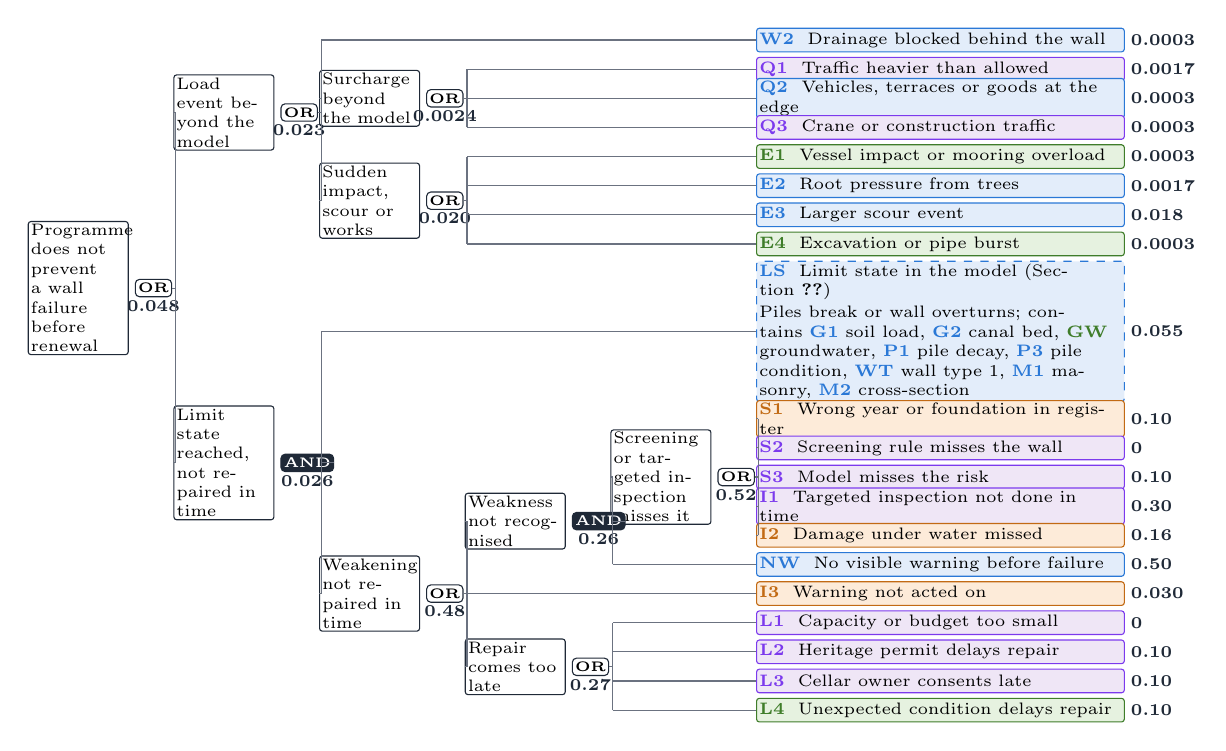
\begin{tikzpicture}[x=1cm,y=1cm,font=\fontsize{6.2}{7}\selectfont,every node/.style={inner sep=1pt}]
\tikzset{gate/.style={draw=ftG,fill=white,rounded corners=1.5pt,font=\fontsize{5}{5}\selectfont\bfseries,minimum width=0.42cm,minimum height=0.22cm},andgate/.style={gate,fill=ftG,text=white},ev/.style={draw=ftG,fill=white,rounded corners=1pt,align=left,text width=1.2cm,minimum height=0.3cm},line/.style={ftL,line width=0.4pt},pv/.style={font=\fontsize{5.6}{6}\selectfont\bfseries,text=ftG}}
\node[draw=ftTb,fill=ftT,rounded corners=1pt,anchor=west,minimum height=0.3cm,text width=4.6cm] at (9.25,0.00) {\textbf{\color{ftTb}W2}\ \ Drainage blocked behind the wall};
\node[pv,anchor=west] at (13.97,0.00) {0.0003};
\node[draw=ftOb,fill=ftO,rounded corners=1pt,anchor=west,minimum height=0.3cm,text width=4.6cm] at (9.25,-0.37) {\textbf{\color{ftOb}Q1}\ \ Traffic heavier than allowed};
\node[pv,anchor=west] at (13.97,-0.37) {0.0017};
\node[draw=ftTb,fill=ftT,rounded corners=1pt,anchor=west,minimum height=0.3cm,text width=4.6cm] at (9.25,-0.74) {\textbf{\color{ftTb}Q2}\ \ Vehicles, terraces or goods at the edge};
\node[pv,anchor=west] at (13.97,-0.74) {0.0003};
\node[draw=ftOb,fill=ftO,rounded corners=1pt,anchor=west,minimum height=0.3cm,text width=4.6cm] at (9.25,-1.11) {\textbf{\color{ftOb}Q3}\ \ Crane or construction traffic};
\node[pv,anchor=west] at (13.97,-1.11) {0.0003};
\node[ev,anchor=west] at (3.70,-0.74) {Surcharge beyond the model};
\node[gate,anchor=west] (g) at (5.06,-0.74) {OR};
\node[pv,anchor=north] at (g.south) {0.0024};
\draw[line] (g.east) -- (5.58,-0.74);
\draw[line] (5.58,-1.11) -- (5.58,-0.37);
\draw[line] (5.58,-0.37) -- (9.25,-0.37);
\draw[line] (5.58,-0.74) -- (9.25,-0.74);
\draw[line] (5.58,-1.11) -- (9.25,-1.11);
\node[draw=ftEb,fill=ftE,rounded corners=1pt,anchor=west,minimum height=0.3cm,text width=4.6cm] at (9.25,-1.48) {\textbf{\color{ftEb}E1}\ \ Vessel impact or mooring overload};
\node[pv,anchor=west] at (13.97,-1.48) {0.0003};
\node[draw=ftTb,fill=ftT,rounded corners=1pt,anchor=west,minimum height=0.3cm,text width=4.6cm] at (9.25,-1.85) {\textbf{\color{ftTb}E2}\ \ Root pressure from trees};
\node[pv,anchor=west] at (13.97,-1.85) {0.0017};
\node[draw=ftTb,fill=ftT,rounded corners=1pt,anchor=west,minimum height=0.3cm,text width=4.6cm] at (9.25,-2.22) {\textbf{\color{ftTb}E3}\ \ Larger scour event};
\node[pv,anchor=west] at (13.97,-2.22) {0.018};
\node[draw=ftEb,fill=ftE,rounded corners=1pt,anchor=west,minimum height=0.3cm,text width=4.6cm] at (9.25,-2.59) {\textbf{\color{ftEb}E4}\ \ Excavation or pipe burst};
\node[pv,anchor=west] at (13.97,-2.59) {0.0003};
\node[ev,anchor=west] at (3.70,-2.04) {Sudden impact, scour or works};
\node[gate,anchor=west] (g) at (5.06,-2.04) {OR};
\node[pv,anchor=north] at (g.south) {0.020};
\draw[line] (g.east) -- (5.58,-2.04);
\draw[line] (5.58,-2.59) -- (5.58,-1.48);
\draw[line] (5.58,-1.48) -- (9.25,-1.48);
\draw[line] (5.58,-1.85) -- (9.25,-1.85);
\draw[line] (5.58,-2.22) -- (9.25,-2.22);
\draw[line] (5.58,-2.59) -- (9.25,-2.59);
\node[ev,anchor=west] at (1.85,-0.92) {Load event beyond the model};
\node[gate,anchor=west] (g) at (3.21,-0.92) {OR};
\node[pv,anchor=north] at (g.south) {0.023};
\draw[line] (g.east) -- (3.73,-0.92);
\draw[line] (3.73,-2.04) -- (3.73,0.00);
\draw[line] (3.73,0.00) -- (9.25,0.00);
\draw[line] (3.73,-0.74) -- (3.70,-0.74);
\draw[line] (3.73,-2.04) -- (3.70,-2.04);
\node[draw=ftTb,fill=ftT,dashed,rounded corners=1pt,anchor=west,align=left,text width=4.6cm] at (9.25,-3.70) {\textbf{\color{ftTb}LS}\ \ Limit state in the model (Section~\ref{sec:prob})\\[1pt]{\fontsize{5.6}{6.6}\selectfont Piles break or wall overturns; contains \textbf{\color{ftTb}G1} soil load, \textbf{\color{ftTb}G2} canal bed, \textbf{\color{ftEb}GW} groundwater, \textbf{\color{ftTb}P1} pile decay, \textbf{\color{ftTb}P3} pile condition, \textbf{\color{ftTb}WT} wall type~1, \textbf{\color{ftTb}M1} masonry, \textbf{\color{ftTb}M2} cross-section}};
\node[pv,anchor=west] at (13.97,-3.70) {0.055};
\node[draw=ftHb,fill=ftH,rounded corners=1pt,anchor=west,minimum height=0.3cm,text width=4.6cm] at (9.25,-4.81) {\textbf{\color{ftHb}S1}\ \ Wrong year or foundation in register};
\node[pv,anchor=west] at (13.97,-4.81) {0.10};
\node[draw=ftOb,fill=ftO,rounded corners=1pt,anchor=west,minimum height=0.3cm,text width=4.6cm] at (9.25,-5.18) {\textbf{\color{ftOb}S2}\ \ Screening rule misses the wall};
\node[pv,anchor=west] at (13.97,-5.18) {0};
\node[draw=ftOb,fill=ftO,rounded corners=1pt,anchor=west,minimum height=0.3cm,text width=4.6cm] at (9.25,-5.55) {\textbf{\color{ftOb}S3}\ \ Model misses the risk};
\node[pv,anchor=west] at (13.97,-5.55) {0.10};
\node[draw=ftOb,fill=ftO,rounded corners=1pt,anchor=west,minimum height=0.3cm,text width=4.6cm] at (9.25,-5.92) {\textbf{\color{ftOb}I1}\ \ Targeted inspection not done in time};
\node[pv,anchor=west] at (13.97,-5.92) {0.30};
\node[draw=ftHb,fill=ftH,rounded corners=1pt,anchor=west,minimum height=0.3cm,text width=4.6cm] at (9.25,-6.29) {\textbf{\color{ftHb}I2}\ \ Damage under water missed};
\node[pv,anchor=west] at (13.97,-6.29) {0.16};
\node[ev,anchor=west] at (7.40,-5.55) {Screening or targeted inspection misses it};
\node[gate,anchor=west] (g) at (8.76,-5.55) {OR};
\node[pv,anchor=north] at (g.south) {0.52};
\draw[line] (g.east) -- (9.28,-5.55);
\draw[line] (9.28,-6.29) -- (9.28,-4.81);
\draw[line] (9.28,-4.81) -- (9.25,-4.81);
\draw[line] (9.28,-5.18) -- (9.25,-5.18);
\draw[line] (9.28,-5.55) -- (9.25,-5.55);
\draw[line] (9.28,-5.92) -- (9.25,-5.92);
\draw[line] (9.28,-6.29) -- (9.25,-6.29);
\node[draw=ftTb,fill=ftT,rounded corners=1pt,anchor=west,minimum height=0.3cm,text width=4.6cm] at (9.25,-6.66) {\textbf{\color{ftTb}NW}\ \ No visible warning before failure};
\node[pv,anchor=west] at (13.97,-6.66) {0.50};
\node[ev,anchor=west] at (5.55,-6.11) {Weakness not recognised};
\node[andgate,anchor=west] (g) at (6.91,-6.11) {AND};
\node[pv,anchor=north] at (g.south) {0.26};
\draw[line] (g.east) -- (7.43,-6.11);
\draw[line] (7.43,-6.66) -- (7.43,-5.55);
\draw[line] (7.43,-5.55) -- (7.40,-5.55);
\draw[line] (7.43,-6.66) -- (9.25,-6.66);
\node[draw=ftHb,fill=ftH,rounded corners=1pt,anchor=west,minimum height=0.3cm,text width=4.6cm] at (9.25,-7.03) {\textbf{\color{ftHb}I3}\ \ Warning not acted on};
\node[pv,anchor=west] at (13.97,-7.03) {0.030};
\node[draw=ftOb,fill=ftO,rounded corners=1pt,anchor=west,minimum height=0.3cm,text width=4.6cm] at (9.25,-7.40) {\textbf{\color{ftOb}L1}\ \ Capacity or budget too small};
\node[pv,anchor=west] at (13.97,-7.40) {0};
\node[draw=ftOb,fill=ftO,rounded corners=1pt,anchor=west,minimum height=0.3cm,text width=4.6cm] at (9.25,-7.77) {\textbf{\color{ftOb}L2}\ \ Heritage permit delays repair};
\node[pv,anchor=west] at (13.97,-7.77) {0.10};
\node[draw=ftOb,fill=ftO,rounded corners=1pt,anchor=west,minimum height=0.3cm,text width=4.6cm] at (9.25,-8.14) {\textbf{\color{ftOb}L3}\ \ Cellar owner consents late};
\node[pv,anchor=west] at (13.97,-8.14) {0.10};
\node[draw=ftEb,fill=ftE,rounded corners=1pt,anchor=west,minimum height=0.3cm,text width=4.6cm] at (9.25,-8.51) {\textbf{\color{ftEb}L4}\ \ Unexpected condition delays repair};
\node[pv,anchor=west] at (13.97,-8.51) {0.10};
\node[ev,anchor=west] at (5.55,-7.96) {Repair comes too late};
\node[gate,anchor=west] (g) at (6.91,-7.96) {OR};
\node[pv,anchor=north] at (g.south) {0.27};
\draw[line] (g.east) -- (7.43,-7.96);
\draw[line] (7.43,-8.51) -- (7.43,-7.40);
\draw[line] (7.43,-7.40) -- (9.25,-7.40);
\draw[line] (7.43,-7.77) -- (9.25,-7.77);
\draw[line] (7.43,-8.14) -- (9.25,-8.14);
\draw[line] (7.43,-8.51) -- (9.25,-8.51);
\node[ev,anchor=west] at (3.70,-7.03) {Weakening not repaired in time};
\node[gate,anchor=west] (g) at (5.06,-7.03) {OR};
\node[pv,anchor=north] at (g.south) {0.48};
\draw[line] (g.east) -- (5.58,-7.03);
\draw[line] (5.58,-7.96) -- (5.58,-6.11);
\draw[line] (5.58,-6.11) -- (5.55,-6.11);
\draw[line] (5.58,-7.03) -- (9.25,-7.03);
\draw[line] (5.58,-7.96) -- (5.55,-7.96);
\node[ev,anchor=west] at (1.85,-5.37) {Limit state reached, not repaired in time};
\node[andgate,anchor=west] (g) at (3.21,-5.37) {AND};
\node[pv,anchor=north] at (g.south) {0.026};
\draw[line] (g.east) -- (3.73,-5.37);
\draw[line] (3.73,-7.03) -- (3.73,-3.70);
\draw[line] (3.73,-3.70) -- (9.25,-3.70);
\draw[line] (3.73,-7.03) -- (3.70,-7.03);
\node[ev,anchor=west] at (0.00,-3.15) {Programme does not prevent a wall failure before renewal};
\node[gate,anchor=west] (g) at (1.36,-3.15) {OR};
\node[pv,anchor=north] at (g.south) {0.048};
\draw[line] (g.east) -- (1.88,-3.15);
\draw[line] (1.88,-5.37) -- (1.88,-0.92);
\draw[line] (1.88,-0.92) -- (1.85,-0.92);
\draw[line] (1.88,-5.37) -- (1.85,-5.37);
\end{tikzpicture}

  \caption{Fault tree for the quay wall programme failing to prevent the failure of a wall before its renewal, as computed for the median wall. OR: at least one input. AND: all inputs together. Numbers: probability of each event and gate, with the load events scaled to the 5.2 years until renewal. The causes inside LS belong to the failure model and are not separate events. Basic events: technical (blue), human (orange), organisational (purple), external (green); bases in Table~\ref{tab:ftprob}.}
  \label{fig:faulttree}
\end{figure}

\subsection{Probabilities of the basic events}\label{sec:ft-probabilities}

Each basic event has a probability for one wall, a range and a basis
(Table~\ref{tab:ftprob}). Of the eight causes inside LS, five are variables of the failure model \parencite{hemel2023,hemel2024}: G1, P1, P3, WT and GW; G2, M1 and M2 enter only through the screen assumption and the model factor $\theta_R$. LS, ``wall reaches a limit state in the model before renewal'', is 0.055 for the median wall (0.15 over 15 years), with a range of 0.033 to 0.46 from the wall being
type~2 or type~1, the largest uncertainty of Section~\ref{sec:dimension-reduction}. The model gives this probability without any
repair and supports only a ranking and an order of magnitude
(Section~\ref{sec:prob-validity}), so using it as a probability is an
assumption. So is spreading the 15-year value evenly over time: the wall type
and the pile condition are a present state, and if the critical load comes
within the exposure, LS approaches 0.15 (Section~\ref{sec:to-results}). The load events are given for 15 years and scaled to the $T_r$ years
until renewal as $1-(1-p)^{T_r/15}$; the human and organisational events are
chances per weakness or per programme and are not scaled. The other events have
one of four bases:
\begin{itemize}
  \item \emph{Data:} S2 is 0, because the screening of
    Section~\ref{sec:approach-selection} flags every wall on its original timber
    piles (Table~\ref{tab:selection}); as the rule was set up on these walls,
    this holds by construction and not for walls elsewhere.
  \item \emph{Derived:} E3 follows from one reported scour case
    \parencite{wijkbericht2024walmuur} among the 51 walls of the register in an
    assumed window of 6 years: $1/(51 \times 6) \times 15 = 0.05$ over 15 years;
    counting only the 19 walls still on timber gives 0.13, near the upper bound.
    L1 follows from the production rate of Section~\ref{sec:regression}: at the
    pace of 2019 to 2026, the 611\,m of the 17 walls are renewed before 2041 in
    more than 99.9\,\% of the bootstrap runs (0.00); only at the lower bound of
    that pace, 22\,m per year, would 45\,\% not be reached.
  \item \emph{Literature:} I2 and I3 are the nominal HEART values for task types C
    (complex, needing skill) and M (miscellaneous)
    \parencite{williams1986heart,heart_table_plos2021}, without error-producing
    conditions; the choice of type is the team's, and plausible conditions would
    raise the top event from 0.049 to 0.052 (Appendix~\ref{app:heart}).
  \item \emph{Assumption:} for the other events no data were found, and the team
    used a fixed scale: extremely rare 0.001, very rare 0.005, rare 0.02,
    occasional 0.10 and likely 0.30. A load event counts only if it occurs
    \emph{and} brings the wall to its limit state; apart from the scour case the
    sources report no such failure, so Q1 and E2 are very rare and the other load
    events extremely rare. NW is 0.5: half of the weak walls are assumed to show
    tilt, cracks or settlement that a regular inspection could see. I1 is 0.30:
    the re-assessment of all quay walls runs until 2030
    \parencite{utrecht_teamchallenge2026}, which covers most of the time until
    renewal, but it need not reach every wall in time; the upper bound, 0.73, is
    the share of the 15-year reference period after 2030 (11 of 15 years).
\end{itemize}

\begin{table}[tbp]
\centering\footnotesize
\caption{Basic events for the median wall. Load events (W2 to E4): probability over 15 years that the event occurs and brings the wall to its limit state, scaled to the years until renewal in the tree. Other events: probability per weakness or per programme.}
\label{tab:ftprob}
\setlength{\tabcolsep}{4pt}
\begin{tabular}{@{}llrll@{}}
\toprule
ID & Event & $p$ & Range & Basis \\
\midrule
LS  & Limit state in the model before renewal & 0.055 & 0.033--0.46 & Model (Sections~\ref{sec:prob}, \ref{sec:regression}) \\
W2 & Drainage blocked & 0.001 & 0.0002--0.005 & Assumption \\
Q1 & Traffic heavier than allowed & 0.005 & 0.001--0.02 & Assumption; occurs \parencite{duic2021} \\
Q2 & Parked vehicles or stored goods & 0.001 & 0.0002--0.005 & Assumption \\
Q3 & Crane or construction traffic & 0.001 & 0.0002--0.005 & Assumption \\
E1 & Vessel hits wall or mooring & 0.001 & 0.0002--0.005 & Assumption \\
E2 & Root pressure & 0.005 & 0.001--0.02 & Assumption; occurs \parencite{duic2020} \\
E3 & Larger scour event & 0.05 & 0.02--0.15 & Derived \parencite{wijkbericht2024walmuur} \\
E4 & Excavation or pipe burst & 0.001 & 0.0002--0.005 & Assumption; occurs \parencite{wijkbericht2025rak5} \\
NW  & No visible warning before failure & 0.50 & 0.30--0.80 & Assumption \\
S1 & Wrong year or foundation in register & 0.10 & 0.05--0.20 & Assumption \\
S2 & Screening rule does not flag wall & 0 & -- & Data (Table~\ref{tab:selection}) \\
S3 & Model misses the risk & 0.10 & 0.05--0.20 & Assumption \\
I1 & Inspection not carried out in time & 0.30 & 0.10--0.73 & Assumption \parencite{utrecht_teamchallenge2026} \\
I2 & Damage under water missed & 0.16 & 0.12--0.28 & HEART type C \parencite{williams1986heart,heart_table_plos2021} \\
I3 & Warning not acted on & 0.03 & 0.008--0.11 & HEART type M \parencite{williams1986heart,heart_table_plos2021} \\
L1 & Capacity or budget too small & 0.00 & 0--0.45 & Derived (Section~\ref{sec:regression}) \\
L2 & Heritage permit delays repair & 0.10 & 0.05--0.20 & Assumption \\
L3 & Cellar owner consents late & 0.10 & 0.05--0.20 & Assumption; occurs \parencite{duic2020} \\
L4 & Unexpected condition delays repair & 0.10 & 0.05--0.20 & Assumption; occurs \parencite{duic2020} \\
\bottomrule
\end{tabular}
\end{table}

Of the 20 events, one comes from the model, one from data, two are derived from
data and two from generic literature; the other 14 are assumptions.
Organisational events such as a delayed permit or a skipped inspection are
recorded only in internal files of the municipality, if at all, and there is no
public register of quay wall incidents; the technical causes with the best
data sit inside LS. The municipality's inspection and incident records,
which it will provide in the case-study phase, or a structured expert judgement would replace
most of them.

\subsection{Propagation and results}\label{sec:ft-results}

For one wall, an OR gate gives $P = 1-\prod_i(1-p_i)$ and an AND gate
$P=\prod_i p_i$ \parencite{vesely1981ftHandbook}. Within one wall, WT and GW sit
inside the model event, where they are drawn once, so their dependence is kept.
For the 17 walls together, each with its own years until renewal and its own LS,
the team used Monte Carlo simulation ($4\times10^5$ runs), because some causes
act on several walls at once. The failure model simulates the walls
independently (Section~\ref{sec:prob-dependence}), so their model events are
linked here with a Gaussian copula and a weak correlation, $\rho=0.084$, a team
judgement for the shared pile age and soil without data.
S3, I1 and I2 are partly shared (the same screening model, programme and
inspectors): 100\,\%, 100\,\% and 50\,\% of their probability is one common draw
for all walls, the rest is drawn per wall. These shares, $\rho$ and the
independence of the load events between walls are assumptions.

For the median wall, the load branch gives 0.023 and ``weakening not repaired in
time'' 0.48. The probability that the programme does not prevent its failure
before renewal is 0.049: 0.015 with all probabilities at their lower bound, 0.47
at their upper bound, where the wall is type~1, and 0.042 to 0.067 over the 17
walls. Without any repair it would be 0.077, so the repair chain lowers it by a
third; if every weakness gave warning (NW~=~0), to 0.039. Over the 17 walls the
expected number of failures before renewal is 0.82
(Figure~\ref{fig:app-fault-tree}). The tree takes the 0.97 model events of
Section~\ref{sec:regression}, lets the repair chain stop half of them, and adds
0.36 from the other load events. Common cause hardly changes the spread
(standard deviation 0.92 to 0.93). Of the 18 minimal cut sets, eight are of order 1
(the load events), five of order 2 (LS with I3 or L1 to L4) and five of order 3
(LS with NW and one of S1 to S3, I1 or I2). The Fussell--Vesely importance
\parencite{fussell1975} is 0.53 for the model event, 0.35 for scour E3, 0.21
for NW, 0.08 for I1 and 0.06 for each of L2 to L4. Moving one probability from
its lower to its upper bound changes the result most for LS (0.20), E3 (0.047)
and L1 (0.013).

\subsection{Interpretation}\label{sec:ft-interpretation}

The results are higher than the incident data suggest. The sources
name about four incidents in the whole Wervengebied between 2017 and 2024: a
temporary support at Oudegracht 110--122 in 2017 \parencite{duic2022}, a partly
closed street on the Kromme Nieuwegracht and a road hole on the Nieuwegracht,
reported in 2020 \parencite{duic2020}, and scour under the wall near the
Bezembrug in 2024 \parencite{wijkbericht2024walmuur}. That is about 0.5 per year
over 4.1\,km of walmuur, or 0.12 per km, all emergency measures, no collapse,
and not all clearly a failure of a walmuur. The tree gives 0.17 per year for the
611\,m of modelled wall, 0.28 per km: more than twice the observed rate.
The incident search was not systematic, so four is a lower bound; the gap fits
a model event on the safe side: the type-1 model is
conservative (Section~\ref{sec:prob-validity}) and 7\,kPa is a heavy load for a
werf (Section~\ref{sec:data-effect}).

The failure model of Section~\ref{sec:prob} gives the technical part of the tree the best support, although its timber properties come from one Amsterdam case; the human part uses generic values and the organisational part mostly
assumptions. A further difficulty was that pile condition is not a yes/no event,
while a missed inspection is; the team used the failure probability of the model
as one event and added NW for the warning it may or may not give. The repair
chain lowers the probability from 0.077 to 0.049, mostly through the targeted
route; the human and organisational events (I1, L2 to L4) matter, but less than
the wall type and scour. Because the range of LS dominates every other swing,
measuring the wall type and the pile condition matters more than speeding up
the repair.

The conclusions hold for the ranking of causes, not for absolute
probabilities. The most useful extra data are the
pile condition from micro-drilling (LS, NW), canal-bed soundings and scour records
(E3), the real programme order (L1 and the years until renewal), and an incident
log of closures and emergency measures to check the result.


% Section 3.2 Trade-off analysis
% Fallback: defines \euro if eurosym is not loaded in the preamble
\providecommand{\euro}{\texteuro}

\section{Trade-off Analysis}
\label{sec:tradeoff}

The team used the fault tree of Section~\ref{sec:fault-tree} to compare
interventions for the median wall until its renewal, 5.2 years at the recent
pace. Each intervention lowers one or more basic events, and the new
probabilities are propagated through the same tree. The decision tree
(Figure~\ref{fig:dtree}) has one decision node with eight alternatives. Seven end
in a chance node with two outcomes: the programme does or does not prevent a
failure, which here means an emergency measure or a closure. The eighth, A7,
first measures the wall and then chooses (a preposterior analysis). The
objective is the lowest expected total cost
\begin{equation}
  E[C_i] = c_i + P_{f,i}\, C_f\, \mathit{DF}_i ,
\end{equation}
where $c_i$ [\euro] is the present value of the cost of intervention $i$, $C_f$
[\euro] the cost of a failure and $\mathit{DF}_i$~\mbox{[--]} the mean discount factor
over the exposure, at 2.8\,\% per year, the standard rate for Dutch social
cost-benefit analyses from 2026 \parencite{discontovoet2025}.

\subsection{Interventions and costs}\label{sec:to-interventions}

Table~\ref{tab:interventions} lists the alternatives: technical, human and
organisational measures, restricting use, renewing now and monitoring.
Strengthening (a relieving floor, new piles or a new screen) is left out: for a
wall renewed within about five years it would cost a large part of a renewal and
then be demolished; for walls that wait much longer it belongs in the tree.
How much a measure lowers an event is not known
from data, so one rule is assumed: a measure moves the events it acts on to the
lower bound of their range in Table~\ref{tab:ftprob}. Two alternatives use the
failure model directly: for A6 it is rerun without surcharge within 1.5\,m of
the edge, which raises $\beta$ of the median wall from 1.05 to 1.31, and for A7
it gives the displacement that a survey would see
(Appendix~\ref{app:prob-checks}). The municipality has high-level unit costs
of replacement \parencite{utrecht_qa2026}; they were not used here, so the
costs below are estimates from published budgets and team judgement in 2026
prices, to be replaced by the municipal figures; cost escalation above
inflation is not modelled and would favour renewing now. Renewing a wall of average length, 36\,m, costs about \euro1.3 million: the programme plan reserves about \euro110 million for the roughly 3\,km of wal- and kluismuren still to be restored, or
\euro35k per metre \parencite{utrecht_programmaplan}. As the wall is renewed
within about five years anyway, renewing now (A4) costs only the present value of bringing that renewal forward, \euro156k, provided extra capacity is
hired; within the same capacity it would delay another wall, which is the order
question of Section~\ref{sec:regression}. The failure cost $C_f = $ \euro1.5
million combines a temporary safety structure of about \euro0.25 million per
wall, from the \euro650k per 100\,m that Amsterdam budgets
\parencite{amsterdam_tender}, \euro0.65 million for the extra cost of an urgent
renewal and \euro0.6 million for closures, damage to cellars and hindrance; as
it is uncertain, it is varied from \euro0.1 to \euro30 million.

\begin{table}[htbp]
\centering
\caption{Decision alternatives for the median wall until its renewal, costed for a wall of average length (36\,m).
T = technical, H = human, O = organisational. New values are lower bounds from
Table~\ref{tab:ftprob}, except those marked *. Costs: one-off plus yearly.}
\label{tab:interventions}
\small
\begin{tabularx}{\textwidth}{@{}llXr@{}}
\toprule
Alternative & Type & Measure and changed basic events & Cost $c_i$ \\
\midrule
A0 Current programme & -- & No extra measures & \euro0k \\
A1 Scour and load control & T & Bed protection and yearly soundings; cameras for the axle limit; root barriers. E3, Q1, E2 & \euro72k + 3k/yr \\
A2 Inspection & H, T & Dive with micro-drilling and a second reviewer; tilt sensors with an alarm. I1, I2, I3, S3; NW 0.50$\to$0.30* & \euro60k + 2k/yr \\
A3 Organisation & O & Share of an extra project leader; agreements with the heritage department and cellar owners; site investigation. L2, L3, L4 & \euro15k + 7k/yr \\
A4 Renew now & T & Renewal in the first year with extra capacity: exposure 5.2$\to$1 year*; E3, W2 & \euro156k* \\
A5 Package & all & A1 + A2 + A3 together & \euro205k \\
A6 Restrict use & O & No terraces, goods or vehicles within 1.5\,m of the edge until renewal. LS 0.055$\to$0.035*; Q1, Q2 & \euro10k + 3k/yr \\
A7 Monitor, then decide & H, T & Survey of the displacement: below 5\,mm keep A0, otherwise A6* & \euro15k (+ A6) \\
\bottomrule
\end{tabularx}
\end{table}

\subsection{Results and preferred alternative}\label{sec:to-results}

Figure~\ref{fig:dtree} gives the results. The
current programme gives $P_f = 0.049$ and an expected cost of \euro68k; $P_f$
has two main parts, the model event that is not repaired in time
($0.055 \times 0.48 = 0.026$) and the load branch (0.023), mostly scour.
Restricting use (A6) lowers $P_f$ by a fifth, to 0.037, at an expected cost of
\euro77k, close to A0. Scour and load control (A1) and inspection (A2) lower it
to 0.035 and 0.041, but cost more than they save. Renewing now (A4) gives the
lowest $P_f$ (0.007). Monitoring (A7) costs \euro83k: the survey finds less
than 5\,mm with probability 0.72, after which $\beta$ rises to 1.54 and the
wall stays in the programme; otherwise $\beta$ falls to 0.36 and use is
restricted.

\begin{figure}[htbp]
\centering
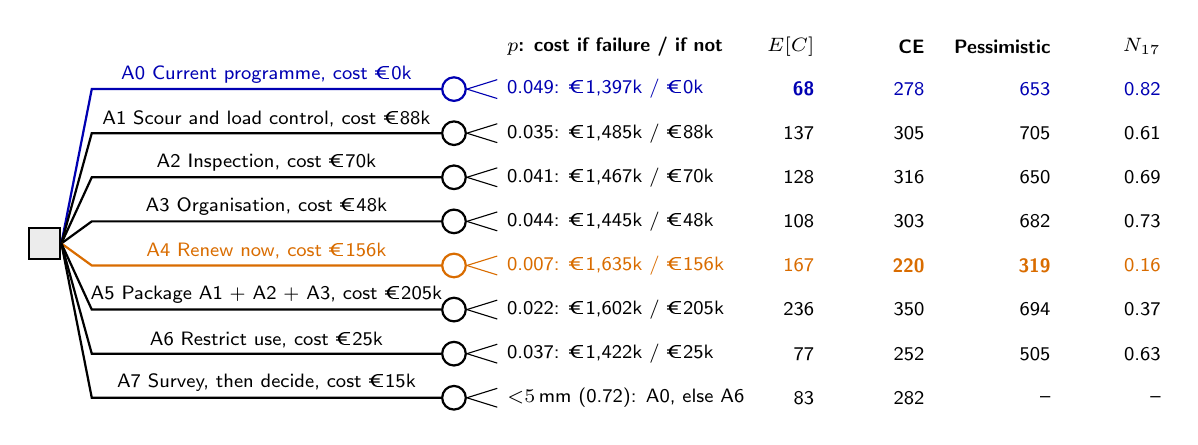
\begin{tikzpicture}[font=\scriptsize\sffamily]
\node[draw, thick, fill=gray!15, minimum size=4mm] (d) at (0,0) {};
\node[right] at (5.75,2.5) {\bfseries $p$: cost if failure / if not};
\foreach \x/\t in {9.9/{$E[C]$}, 11.3/{CE}, 12.9/{Pessimistic}, 14.3/{$N_{17}$}}
  \node[left] at (\x,2.5) {\bfseries \t};
\foreach \idx/\alt/\cst/\pf/\cf/\cn/\ec/\ce/\pe/\n/\col in {
  0/A0 Current programme/0/0.049/1{,}397/0/\textbf{68}/278/653/0.82/blue!70!black,
  1/A1 Scour and load control/88/0.035/1{,}485/88/137/305/705/0.61/black,
  2/A2 Inspection/70/0.041/1{,}467/70/128/316/650/0.69/black,
  3/A3 Organisation/48/0.044/1{,}445/48/108/303/682/0.73/black,
  4/A4 Renew now/156/0.007/1{,}635/156/167/\textbf{220}/\textbf{319}/0.16/orange!85!black,
  5/A5 Package A1 + A2 + A3/205/0.022/1{,}602/205/236/350/694/0.37/black,
  6/A6 Restrict use/25/0.037/1{,}422/25/77/252/505/0.63/black} {
  \pgfmathsetmacro{\y}{1.96-0.56*\idx}
  \node[draw, thick, circle, minimum size=3mm, inner sep=0pt, \col] (c\idx) at (5.2,\y) {};
  \draw[thick, \col] (d.east) -- (0.6,\y) -- node[above=-1.5pt] {\alt, cost \euro\cst k} (c\idx.west);
  \draw[\col] (c\idx.east) -- (5.75,\y+0.12);
  \draw[\col] (c\idx.east) -- (5.75,\y-0.12);
  \node[right, \col] at (5.75,\y) {\pf: \euro\cf k / \euro\cn k};
  \node[left, \col] at (9.9,\y) {\ec};
  \node[left, \col] at (11.3,\y) {\ce};
  \node[left, \col] at (12.9,\y) {\pe};
  \node[left, \col] at (14.3,\y) {\n};
}
\pgfmathsetmacro{\y}{1.96-0.56*7}
\node[draw, thick, circle, minimum size=3mm, inner sep=0pt] (c7) at (5.2,\y) {};
\draw[thick] (d.east) -- (0.6,\y) -- node[above=-1.5pt] {A7 Survey, then decide, cost \euro15k} (c7.west);
\draw (c7.east) -- (5.75,\y+0.12);
\draw (c7.east) -- (5.75,\y-0.12);
\node[right] at (5.75,\y) {${<}5$\,mm (0.72): A0, else A6};
\node[left] at (9.9,\y) {83};
\node[left] at (11.3,\y) {282};
\node[left] at (12.9,\y) {--};
\node[left] at (14.3,\y) {--};
\end{tikzpicture}
\caption{Decision tree for the median wall until its renewal, with the results.
Square: decision node; circle: chance node with the probability $p$ that the
programme does not prevent a failure, from the fault tree of
Section~\ref{sec:fault-tree} with the changed basic events. Costs in \euro k,
present values at 2.8\,\%; $C_f = $ \euro1{,}500k. CE: certainty equivalent with
exponential utility, $R = $ \euro0.5 million. Pessimistic: $E[C]$ with all basic
events at the upper bound of their range in Table~\ref{tab:ftprob} and LS at its
type-1 value ($p$ of A0 0.47); a measure lowers an event by the same factor as
in the base case (assumption). $N_{17}$: expected number of failures among the
17 walls before renewal. Bold: lowest cost per criterion; blue: preferred when
risk-neutral; orange: preferred under both risk-averse criteria.}
\label{fig:dtree}
\end{figure}

A risk-neutral decision maker looks only at $E[C]$, which with $C_f = $ \euro1.5 million favours A0, with A6
\euro9k behind. The choice depends on $C_f$ (Figure~\ref{fig:app-fault-tree}): A6 is the cheapest from
\euro2.4 million, A7 from \euro4.4 million and A4 from \euro5.05 million. A public
owner of heritage walls is more likely risk-averse, which the team tested in two
ways. With an exponential utility function,
$\mathrm{CE} = R \ln E[e^{C/R}]$ with risk tolerance $R = $ \euro0.5 million
(assumption), renewing now has the lowest certainty equivalent (\euro220k
against \euro252k for A6 and \euro278k for A0), because it almost removes the
large loss; with $R = $ \euro1 million A6 is best and with \euro2 million A0.
In a pessimistic scenario with all events at their upper bound and the wall of
type~1, A4 is also the cheapest (\euro319k against \euro505k for A6). The
risk-neutral choice is therefore A0, followed by A6, and the risk-averse choice
A4. These choices depend on the absolute level of $P_f$, which the model does
not give (Section~\ref{sec:prob-validity}). With event LS three times lower, A0
stays the cheapest; with LS three times higher, or without spreading the
15-year value over time (LS = 0.15), A6 becomes the cheapest (\euro124k and
\euro116k against \euro140k and \euro127k for A0). A4 keeps the lowest
certainty equivalent in every case.

The median wall is orange, so Table~\ref{tab:walls-decision} repeats the decision, with the same costs, for a red wall that is probably type~1, Oude Gracht Rak~03
OZ, and for the green wall with the lowest $P_f$, Kromme Nieuwe Gracht 003. For
the red wall, renewed in about 2.6 years, restricting use is already the
cheapest at the base $C_f$ and renewing now is the risk-averse choice; for the
green wall the current programme stays the cheapest up to \euro3.95 million.
This backs the measures per class of Section~\ref{sec:approach-selection}:
restricted use and early renewal for red walls, regular inspection for green
ones.

\begin{table}[htbp]
\centering
\small
\caption{Decision for three walls until their renewal, with the costs of
Table~\ref{tab:interventions}, $C_f = $ \euro1.5 million and $R = $ \euro0.5
million. $T_r$: years until renewal; $C_f^{*}$: failure cost from which
restricting use (A6) is the cheapest.}
\label{tab:walls-decision}
\setlength{\tabcolsep}{4pt}
\begin{tabular}{@{}l l r r c l l r@{}}
\toprule
Wall & Class & $T_r$ [yr] & $P_f$ A0 & $E[C]$ A0 / A6 / A4 [\euro k] & Cheapest & Lowest CE & $C_f^{*}$ [\euro M] \\
\midrule
OG Rak 03 OZ & red & 2.6 & 0.067 & 98 / 95 / 109 & A6 & A4 & 1.3 \\
OG Rak 09 WZ (median) & orange & 5.2 & 0.049 & 68 / 77 / 167 & A0 & A4 & 2.4 \\
KNG 003 & green & 6.7 & 0.044 & 60 / 77 / 209 & A0 & A6 & 3.95 \\
\bottomrule
\end{tabular}
\end{table}

\subsection{Monitoring and the value of information}\label{sec:to-monitoring}

The municipality named monitoring as a source of evidence
\parencite{utrecht_qa2026}. In the model, a type-1 wall has moved 6 to 9\,mm under its soil and water and a type-2 wall 1 to 3\,mm, so a
survey of the horizontal displacement, with an error of 2\,mm, mainly reveals
the wall type, much as a survived load of 10\,kN/m$^2$ with small displacements
raised $\beta$ from 1.5 to 3.2 in \textcite{hemel2024}. For the median wall the survey is worth
nothing before its cost of \euro15k, because the wall is renewed within about
five years and restricting use is a cheap response anyway. For a wall that has
to wait 15 years, as most of the 60\,km will, the same survey is worth \euro3k
at $C_f = $ \euro1.5 million but \euro56k at \euro5 million. Monitoring thus pays
where renewal is far away, which is where the portfolio method uses it
(Section~\ref{sec:approach-selection}). Satellite data measure vertical
movement, which belongs to the settlement mechanism that the model leaves out;
they serve as an indicator, not as an update of $\beta$.

\subsection{Reflection}\label{sec:to-reflection}

The team expected the organisational measures to matter more. They lower $P_f$
by a tenth (A3), because the targeted route already stops half of the failures
of the model and the rest comes from the wall type and scour. The team did not expect restricting use to compete with the
current programme, nor renewing now to win under risk aversion. Both
follow from the short exposure, which favours measures that work at once over
measures whose benefit builds up over years, such as bed protection or an extra
project leader. Not all objectives can be put in euros. $C_f$ has no life-safety
part: on a busy werf, an expected 0.05 fatalities per failure at a value of a
statistical life of about \euro2.2 million in 2001 prices \parencite{deblaeij2003},
some \euro3.5 million today, would add about \euro0.18 million, still below the
\euro2.4 million at which A6 becomes the cheapest. The cost of A6
falls mostly on terrace owners, who lose seats by the water, and the closures
of A4 hinder access to the inner city; these conflicts are not in $C_f$ and need
a political choice.

The inputs differ in quality. Event LS comes from the failure model, whose
inputs are mostly literature values; NW and the organisational events are
assumptions; the effect of A6 is as uncertain as the surcharge itself, and
scour E3 rests on a single case. The costs are team estimates: for the median
wall, a measure would match A0 at \euro15k for restricting use (estimate
\euro25k) but at \euro7k to \euro18k for A1 to A3 (estimates \euro48k to
\euro88k); with all costs of the measures halved A6 becomes the cheapest, and
with a renewal cost 30\,\% higher A6 replaces A4 as the risk-averse choice.
The ranking of the alternatives therefore holds only within the tested range:
A0 and A6 swap places when LS is three times higher or A6 is cheaper, and A4
stays the risk-averse choice unless renewal costs more. The conclusions assume
independent walls, measures that work as soon as they are taken, the
lower-bound rule for their effect, and a renewal within about five years; with
half that effect, A0 stays the cheapest and A6 second (\euro85k).
Because the measures interact through the AND and OR gates, they have to be
judged together, as in A5. The data that would help most are the municipal unit
costs and the costs of emergency measures in Utrecht, to fix $C_f$ and the
costs of the measures; canal
soundings and a scour record, to estimate E3; how often weak walls in Utrecht
showed warning signs, to estimate NW; and the wall type per wall, which would
allow renewing early only the weak type-1 walls.

\subsection{Effectiveness of the interventions}\label{sec:to-effectiveness}

Measured against the current programme, no measure pays for itself in expected
value at $C_f = $ \euro1.5 million for the median wall, whereas restricting use
does for a red wall such as Rak~03 OZ. For the median wall it comes closest: it lowers $P_f$ by a fifth for
\euro25k, under 2\,\% of the cost of a renewal. Renewing now lowers it by 85\,\%
for an extra \euro156k and the package by 55\,\% for \euro205k, whereas
inspection and organisation, at 15 and 10\,\%, are not effective on their own.
For walls renewed within a few years, the effective measures are those that
act at once: restricting use on the red walls, and renewing the weakest first
when extra capacity is available. Monitoring becomes effective for walls that
will wait much longer.

The largest lever is the pace of the programme
(Section~\ref{sec:regression}). Returning to the pace of 2015 to 2018 brings the
renewal of the 17 walls forward, which costs \euro1.2 million in present value
at \euro35k per metre, and avoids 0.42 expected limit states, worth
\euro0.6 million at $C_f = $ \euro1.5 million: it pays only from $C_f \approx$
\euro3 million. At the base failure cost, budget and the accessibility of the city centre, rather than this risk, should set the pace.



%% ----------------------------------------------------------------------
%%  MAX 3 PAGES
%%
%%  TASK DESCRIPTION
%%  The 'rich' undesired event broken down in Section
%%  \ref{sec:fault-tree} is used here to analyse the possible
%%  interventions that reduce its occurrence probability. You may consider
%%  interventions from a technical, human factors and/or organisational
%%  perspective. Creativity and research initiative are appreciated here.
%%  Structure and systematically investigate the interventions in a
%%  decision tree in order to compare the costs and benefits of your
%%  decision alternatives.
%%  Present and interpret the results. For example: do the results
%%  correspond to your beliefs? What are the most effective interventions
%%  in your system? What other data would be needed to elaborate the
%%  decision tree further? Which decision alternative is preferred from a
%%  rational risk-neutral optimisation procedure, and which from a
%%  risk-averse procedure?
%%  Reflect on the procedure and the results. Can all conflicting
%%  objectives be quantified? Discuss the main difficulties encountered
%%  with trading off the objectives and processing the data. Explain to
%%  what extent data availability or quality issues may have impacted your
%%  analysis, reflect on the role of technical, human and organisational
%%  factors, and state under what conditions conclusions can be drawn from
%%  the optimal interventions and the collected data.
%%  To what extent are the proposed intervention measures effective in
%%  reducing the occurrence frequency of undesired events?
%%
%%  CHECKLIST (challenge task 6: compare interventions and programme them
%%  under real constraints)
%%   - Structure the full range of alternatives: doing nothing and
%%     continuing to monitor; restricting use (load limits, traffic
%%     restrictions, closure); maintenance that preserves existing
%%     functionality; life-extension and strengthening (renovation,
%%     foundation improvement, relieving structures, load reduction);
%%     replacement at the end of life; and improvement or expansion that
%%     adds functionality, such as nature-friendly banks, ecological
%%     integration, circular or demountable structures, and climate
%%     adaptation.
%%   - Weigh these against annual budget, contractor and engineering
%%     capacity, permissible disruption and accessibility, heritage
%%     requirements, dependency on private owners, coordination with other
%%     works, and financial risks including inflation, cost escalation and
%%     the discount rate applied to long-lived public investments.
%% ----------------------------------------------------------------------
